\documentclass[10pt, letterpaper]{article}
% \documentclass[10pt,twocolumn,letterpaper]{article}
% \usepackage[a4paper, total={6in, 8in}]{geometry}
\usepackage{cvpr}
\usepackage{times}
\usepackage{epsfig}
\usepackage{graphicx}
\usepackage{amsmath}
\usepackage{amssymb}
\usepackage{enumitem}
\usepackage{url}
\usepackage{mathrsfs}
\usepackage{float}
\usepackage{amsfonts,nicefrac,mathtools,bbm,color}
\usepackage{verbatim}

\newcommand{\real}{\mathbb{R}}

\newcommand{\bsx}{\boldsymbol{x}}

\newcommand{\e}{\mathbb{E}}
\newcommand{\var}{\mathrm{var}}

\newcommand{\rct}{\mathcal{R}}
\newcommand{\odb}{\mathcal{O}}

\newcommand{\err}{\varepsilon}

\renewcommand{\le}{\leqslant}
\renewcommand{\ge}{\geqslant}

\newcommand{\tran}{\mathsf{T}}

\newcommand{\simiid}{\stackrel{\mathrm{iid}}\sim}

\newcommand{\rd}{\,\mathrm d}

% Specialized notation. 
% Small roman subscripts are more readable than smal italic ones.

\renewcommand{\k}{\mathrm{k}}
\renewcommand{\r}{\mathrm{r}}
\newcommand{\s}{\mathrm{s}}
\renewcommand{\o}{\mathrm{o}}

\newcommand{\rk}{\mathrm{rk}}
\newcommand{\rkt}{\mathrm{rkt}}
\newcommand{\rkc}{\mathrm{rkc}}
\newcommand{\rt}{\mathrm{rt}}
\newcommand{\rc}{\mathrm{rc}}

\newcommand{\ok}{\mathrm{ok}}
\newcommand{\okt}{\mathrm{okt}}
\newcommand{\okc}{\mathrm{okc}}

\newcommand{\ot}{\mathrm{ot}}
\newcommand{\oc}{\mathrm{oc}}

\newcommand{\sk}{\mathrm{sk}}
\newcommand{\skt}{\mathrm{skt}}
\newcommand{\skc}{\mathrm{skc}}

\newcommand{\st}{\mathrm{st}}
\renewcommand{\sc}{\mathrm{sc}}


\newcommand{\nr}{n_{\r}}
\newcommand{\nrk}{n_{\rk}}
\newcommand{\nrkt}{n_{\rkt}}
\newcommand{\nrkc}{n_{\rkc}}

\newcommand{\nrt}{n_{\rt}}
\newcommand{\nrc}{n_{\rc}}


\newcommand{\no}{n_{\o}}
\newcommand{\nok}{n_{\ok}}
\newcommand{\nokt}{n_{\okt}}
\newcommand{\nokc}{n_{\okc}}

\newcommand{\fr}{f_{\r}}
\newcommand{\fo}{f_{\o}}

\newcommand{\byr}{\bar Y_{\r}}
\newcommand{\byrk}{\bar Y_{\rk}}
\newcommand{\byrkt}{\bar Y_{\rkt}}
\newcommand{\byrkc}{\bar Y_{\rkc}}

\newcommand{\byrt}{\bar Y_{\rt}}
\newcommand{\byrc}{\bar Y_{\rc}}

\newcommand{\byo}{\bar Y_{\o}}
\newcommand{\byok}{\bar Y_{\ok}}
\newcommand{\byokt}{\bar Y_{\okt}}
\newcommand{\byokc}{\bar Y_{\okc}}

% Include other packages here, before hyperref.

% If you comment hyperref and then uncomment it, you should delete
% egpaper.aux before re-running latex.  (Or just hit 'q' on the first latex
% run, let it finish, and you should be clear).
\usepackage[breaklinks=true,bookmarks=false]{hyperref}

\cvprfinalcopy % *** Uncomment this line for the final submission

\def\httilde{\mbox{\tt\raisebox{-.5ex}{\symbol{126}}}}

% Pages are numbered in submission mode, and unnumbered in camera-ready
%\ifcvprfinal\pagestyle{empty}\fi
\setcounter{page}{1}
\begin{document}

%%%%%%%%% TITLE
\title{Using Poisson Binomial GLMs to Reveal Voter Preferences}

\author{Evan Rosenman\\
Stanford University\\
{\tt\small rosenman@stanford.edu}
% For a paper whose authors are all at the same institution,
% omit the following lines up until the closing ``}''.
% Additional authors and addresses can be added with ``\and'',
% just like the second author.
% To save space, use either the email address or home page, not both
\and
Nitin Viswanathan\\
Stanford University\\
{\tt\small nviswana@stanford.edu}
}

\maketitle
%\thispagestyle{empty}

%%%%%%%%% ABSTRACT
% \begin{abstract}
% TODO
% \end{abstract}

%%%%%%%%% BODY TEXT

\section{Abstract}

\section{Introduction}
Political organizations seek to build voting models to explain individual voter preferences, as this information is vital for voter targeting. For example, they want to identify swing voters and split ticket voters (who voted for candidates across multiple political parties) to focus outreach efforts for future elections.

In the US, voting data indicating how many votes every candidate receives is available at the precinct level, but the most granular data – who voted for which candidate – is private. As a result, political groups are forced to rely on polling data to perform analysis at the individual voter level. However, polling has not been correct in several recent elections, most notably the 2016 presidential election. Polling data can not only be unreliable but it is also incomplete, as voters are not obligated to express their true preferences and the majority of voters will not participate in polls. We develop individual voter models based off of publicly available precinct-level voting data.

Using precinct-level data, we develop a new type of GLM to explain individual voter behavior in Pennsylvania for the 2016 presidential election. We focus on predicting votes for both Hillary Clinton and Donald Trump in the state of Pennsylvania as it was a key swing state that went in favor of Donald Trump in the 2016 presidential election. Trump's margin of victory was very slim at only 44,292 votes, only 0.72\% more than Clinton's \cite{NYT}. Precinct-level election results are the most granular results available; for reference there are about 9,000 precincts total in Pennsylvania \cite{NYT}. 

We formulate the problem using a Poisson binomial generalized linear model, which has not to our knowledge been done before in other literature. We then minimize the negative log-likelihood via batch gradient descent.

Our paper makes two key contributions:
\begin{itemize}[noitemsep]
	\item We develop the math necessary to use and train Poisson binomial GLMs
	\item We apply poission binomial GLMs to the specific task of revealing voter preferences
\end{itemize}

\section{Related Work}
Theoretical work on the Poisson Binomial distribution has focused on computationally tractable ways to estimate its distribution function, often via approximations to other distributions 
\cite{EHM19917, roos1999, chen1974}. Prior research \cite{HONG201341} has identified a closed-form expression for the CDF, which relies on the discrete Fourier Transform. This technique is leveraged in the \texttt{poibin} package \cite{PoibiGithub}, which we use for this project. The application of the Poisson Binomial distribution to the generalized linear model setting has been discussed by Chen and Liu \cite{Poibi}, who propose it for hypothesis testing on the parameter vector for a logistic regression model. But we find no references in the literature to our approach: building generalized linear models for Poisson Binomial-distributed sums. 

There is a richer body of literature on our chosen application: modeling voter preferences in elections. This research separates into two primary methodologies. In the first, researchers are interested in the relationship between voter characteristics and their ballot preferences. To obtain labeled datasets, researchers make use of voter surveys \cite{dubrow2007choosing}, exit polls \cite{carsey1995contextual}, or modeling whether an individual voted (which is public record), rather than her choice of candidate \cite{rusch2013influencing}. They then fit models via simple GLMs, like the multinomial probit or multinomial logit model, which ``represent voter choice as a decision among unordered alternatives (parties, candidates) as a function of chooser (voter) and choice (party/candidate) attributes" \cite{DOW2004107}. 

In the second methodology, researchers are interested in the relationship between candidate characteristics or voting methods and vote outcomes. In these studies \cite{miller1998impact, frisina2008ballot, 10.2307/24371899}, researchers frequently use aggregate vote totals from precincts, counties, or states. Relationships are then uncovered by standard regression techniques, like linear mixed models \cite{10.2307/2585758} AAAAADDDSDFSDFSDFSDFSDF . Closely related to this literature is the approach of popular election prognosticators like FiveThirtyEight \cite{538} to model election outcomes using a mix of polling and demographic data. 

\section{Dataset}

\subsection{Overview}

We combined two disparate datasets for our project. \\

\noindent \textbf{Pennsylvania precinct-level election results} \\
Our dataset of Pennsylvania precinct-level election results contains the total number of votes received by each candidate by precinct in the 2016 presidential election. We obtained this dataset from OpenElections \cite{OpenElections}.

\begin{table}[H]
\begin{center}
\begin{tabular}{ |l|l|l|l| } 
\hline
County Name & Precinct Name & Candidate Name & Number of votes \\
\hline \hline
MONTGOMERY & ABINGTON W1 D1 & HILLARY CLINTON & 603  \\
\hline
MONTGOMERY & ABINGTON W1 D1 & DONALD TRUMP & 388  \\
\hline
... & ...& ... & ...  \\
\hline
\end{tabular}
\end{center}
\end{table}

\noindent \textbf{Pennsylvania voter file} \\
Our other dataset is the Pennsylvania voter file which we obtained directly from the Pennsylvania Department of State \cite{PAVoterFile}. This dataset contains a row for every registered voter in Pennsylvania as well as their party registration, limited demographic information (age, gender), and voting participation over a set of recent primaries and general elections.
\begin{table}[H]
\begin{center}
\begin{tabular}{ |l|l|l|l|l|l| } 
\hline
County Name & Precinct Name & Voter Name & Gender & Age & Other Attributes \\
\hline \hline
MONTGOMERY & ABINGTON 1-1 & Jane Doe & Female & 27 & ... \\
\hline
... & ... & ... & ... & ... & ... \\
\hline
\end{tabular}
\end{center}
\end{table}

\subsection{Dataset Preparation and Validation}

Because these files were sourced from two different datasets, we ran into some challenges in cleanly mapping them with each other. In particular, there is no shared precinct identifier across the files - precinct names often did not match between the files as in the above tables, and there was no other common precinct identifier. As a result, we had to review over 9,000 precincts manually to determine the best way to match them between the files. If either the voter file or precinct-level results were corrupted or did not match which each other, we removed the entire county from our dataset.

After our data cleaning, filtering, and mapping, we ended up with a dataset of 48 of Pennsylvania's 67 counties. Together, these counties represent 6,837 precincts and about 4.07 million total votes for Clinton and Trump. This corresponds to about 66\% of voters in Pennsylvania. The sample had a small pro-Clinton bias, with $52.1\%$ of the voters who cast a major-party ballot supporting Clinton in our sample, versus 49.6\% statewide. 

We only model based on the vote counts for Hillary Clinton and Donald Trump because about 96\% of votes went for one of them. We examined this further and saw that the sum of Clinton/Trump votes in some precincts is not equal to the total number of votes cast, but is within 10\% in most cases. To address this, we take the percentage of Clinton/Trump votes cast in a precinct went to Clinton and multiply it by the total number of Clinton/Trump votes in the precinct, and repeat this for Trump. This is our estimate of how many voters in a precinct would have went for Clinton/Trump if these two candidates were the only two options.

\section{Methods}

\subsection{Poisson Binomial GLM}

We use a Generalized Linear Model based on the Poisson binomial distribution. We model an individual $i$ voting for Clinton as a Bernoulli random variable, so $p_i = \sigma(\theta^TX_i)$, where $\sigma(.)$ denotes the sigmoid function, $\theta$ is a set of parameters to fit, and $X_i$ are known covariates for voter $i$ from the Pennsylvania voter file. Note that the probability of an not voting for Clinton (i.e. voting for Trump) is $1 - p_i$. We assume that these Bernoulli random variables are independent but not necessarily identically distributed, since we expect that different voters would have different probabilities of voting for Clinton.

Combining this representation of a voter with the fact that in a given precinct we know the total number of votes for Clinton and Trump, the total number of Clinton voters in each precinct will follow a Poisson binomial distribution, which is the probability distribution of a sum of independent but not necessarily identically distributed Bernoulli random variables \cite{Poibi}. For a precinct $k$ with $D$ votes for Clinton out of $T$ total votes, the likelihood is given by:

$$\ell_k(\theta) = \sum_{A \in F_k} \prod_{i \in A} p_i \prod_{j \in A^c}(1 - p_j)$$
where $F_k$ is the set of all configurations of $T$ votes in which a total of $D$ votes were cast for Clinton; $A$ is the set of voters who voted for Clinton under that configuration, and $A^c$ is the set of voters who voted for Trump under that configuration. The likelihood of the precinct-level results given parameters $\theta$ can be calculated by multiplying the likelihoods from every precinct together:

$$\ell(\theta) = \prod_k \ell_k(\theta)$$

In order to determine the optimal parameters $\theta$, we need to maximize this likelihood over the Pennsylvania precincts. Note that the Poisson binomial likelihood involves sums over all possible configurations of votes -- e.g. if Clinton received 200 out of 500 total votes in a precinct, then the likelihood involves a sum over $500 \choose 200$ configurations. Although we can directly estimate the likelihood using the \texttt{poibin} package, calculating the gradient is computationally infeasible.

\subsection{Calculating the Gradient}

To address this problem, we make use of the Lyapunov CLT \cite{LyapunovCondition} to observe that the asymptotic distribution of $d_k$, the number of votes for Clinton in precinct $k$, is given by: 
\[ d_k \stackrel{d} \longrightarrow N \left(\sum_{i} p_{k,i}, \sum_{i} p_{k, i}(1-p_{k, i}) \right) \] 
where $p_{k, i}$ is the $i^{th}$ entry of $p_k$. This result is proven in the appendix. It allows us to \emph{estimate} the likelihood with a much simpler function of $\theta$. In this case, the contribution of precinct $k$ to the overall log-likelihood is approximately: 
\[ \ell_k = -log \left( \phi_k\right) + \frac{1}{\phi_k^2} \left( d_k -\mu_k \right)^2  \] 
where irrelevant constants have been dropped, $\mu_k =  \sum_{i} p_{k, i}(1-p_{k, i}), \phi_k^2 = \sum_{i} p_{k, i}(1-p_{k, i})$, and $p_{k, i} = \sigma(\theta^T x_{k, i})$. This yields a gradient of the form: 
\begin{align*}
\nabla_{\theta} \ell_k &=  -\frac{1}{2} \left(\frac{(d_k - \mu_k)^2}{\phi^4} - \frac{1}{\phi^2} \right) \left( \sum_{i} (2 p_{k, i} - 1)(1-p_{k, i})p_{k, i}x_{k, i} \right) + \frac{1}{\phi^2} (d_k - \mu_k) \left( \sum_i p_{k, i} (1 - p_{k, i}) x_{k, i} \right)
\end{align*}

\subsection{Neural Net} 
As one potential improvement to our modeling, we considered using a neural net -- rather than a simple logistic regression -- to relate individual-level covariates to the probability of voting for Clinton. In particular, our new model for $p_{k, i}$, the Clinton-voting probability for person $i$ in precinct $k$, is given by: 
\begin{align*}
h_{k, i} &= \sigma\left(W_1 x_{k, i} + b_1 \right) \\
p_{k, i} &= \sigma\left(W_2 h_{k, i} + b_2 \right) 
\end{align*}
where $x_{k, i}$ are the covariates for the individual. Denoting $\mu_k = \sum_{i = 1}^{n_k} p_{k, i}$ and $\sigma_k^2 = \sum_{i = 1}^{n_k} p_{k, i} (1 - p_{k, i})$ where $n_k$ is the number of votes cast in precinct $k$, we see: 

\begin{align*}
\frac{\partial \ell_k}{\partial p_{k, j}} &= - \frac{1 - 2p_{k, j}}{2 \sigma_k^2} + \frac{1 - 2p_{k, j}}{2 \sigma_k^4} (d_k - \mu_k)^2  + \frac{1}{\sigma_k^2} \left(d_k - \mu_k \right) \\
\frac{\ell_k}{\partial b_2} &= \sum_{j = 1}^{n_k} \frac{\partial \ell_k}{\partial p_{k, j}} \cdot p_{k, j} (1 - p_{k, j}) \\
\frac{\ell_k}{\partial W_2} &= \left\{ h_{k, j} \right\}_j^T \left\{ \frac{\partial \ell_k}{\partial p_{k, j}} \cdot p_{k, j} (1 - p_{k, j})\right\}_{j} \\
\frac{\ell_k}{\partial b_1} &= \sum_{j = 1}^{n_k} \left\{ \frac{\partial \ell_k}{\partial p_{k, j}} \cdot p_{k, j} (1 - p_{k, j})\right\}_{j} W_2^T \circ \left\{ h_{k, j}(1 - h_{k, j})\right\}_j \\
\frac{\ell_k}{\partial W_1} &= \left\{ x_{k, j} \right\}_j^T \left\{ \frac{\partial \ell_k}{\partial p_{k, j}} \cdot p_{k, j} (1 - p_{k, j})\right\}_{j} W_2^T \circ \left\{ h_{k, j}(1 - h_{k, j})\right\}_j
\end{align*}
where $\{x_j\}_j$ denotes a column vector consisting of the entries $x_j$ and $\circ$ denotes a Hadamard product. We implement these gradients and train our new neural net

\subsection{Optimization Methodology}

Our goal is to fit one set of parameters $\theta$ such that for voter $i$ with features $X_i$, $p_i = \sigma(\theta^TX_i)$ is an accurate representation of their probability of voting for Clinton. We train our model using gradient descent on the negative log-likelihood of our Poisson binomial distribution, where the log-likelihood and gradient functions are as defined in section 5.1. For each training epoch, we train our model on every precinct in the training set, updating parameter values after each precinct. We explored using batch and stochastic gradient descent, but both of these resulted in slower convergence.

We initialized all of our parameters to 0, which meant that at the beginning we were assuming that every voter had a 50\% chance of voting for Clinton. We experimented with regularization, but did not find it necessary as we were not having issues overfitting to the training set and adding regularization did not noticeably impact our model's performance on our holdout. 

One specific issue we ran into when running gradient descent was extremely large or small gradients (that often returned as $NaN$ due to underflow issues). We found the best way to handle these gradients was to ignore the counties with extremely small gradients as they would not have changed the likelihood at all and to cap large gradients if they were beyond a certain magnitude.

With the above methodology, we consistently reached convergence within 20 epochs when training our models.

\section{Experiments}

We had two main goals with our experiments. First, we wanted to show that our model was accurate in predicting voter preferences. We did this by training our model on 70\% of the counties in our dataset and evaluating it on the remaining 30\% in different ways. Secondly, once we were convinced that our model was accurate, we trained our model on the entire dataset to obtain a comprehensive voting model and checked it against accepted beliefs around voter preferences.

NITIN TODO - We evaluated our model in a few different ways. Explain each of the 3 eval techniques (holdout $R^2$, weak labeling with landslides, weak labeling based on vote in primary)

\section{Results \& Analysis}

TODO - subsection for each experiment we ran with a summary and explanation of the results.



\section{Results}

Using stochastic gradient ascent, we fit a simple model to the four counties where we predict the probability to vote for Clinton given county, party registration, primary participation, gender, and age. Computing the log-likelihood every 25 iterations, we see a modest improvement over the first 400 iterations (after which the log-likelihood plateaus): 
\begin{figure}[H]
\centering
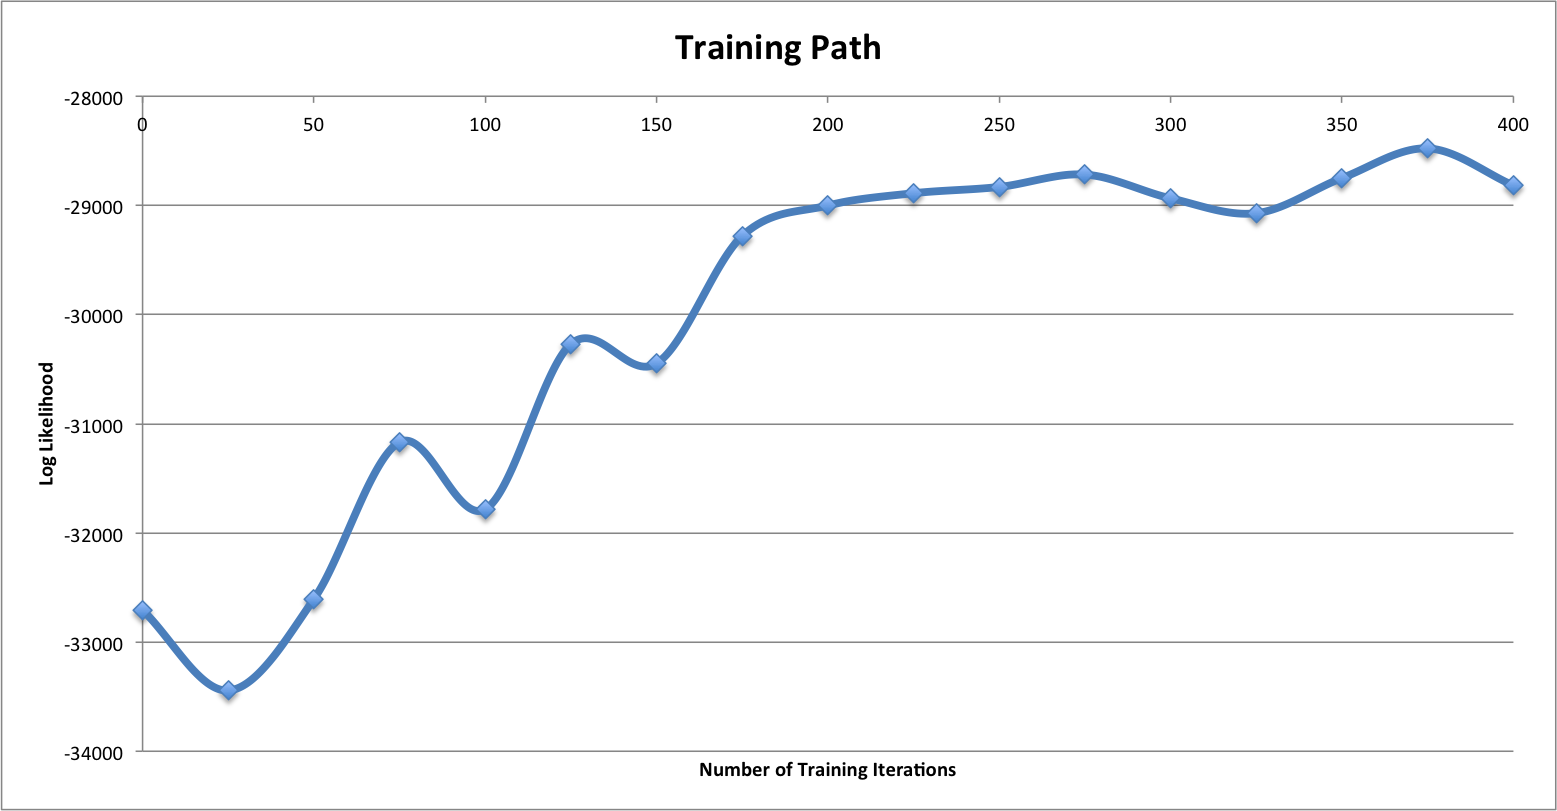
\includegraphics[scale = 0.4]{TrainingPath}
\end{figure}

Below we present the coefficients coming out of the model, noting that positive values indicate that a voter is more likely to vote for Clinton over Trump:

\begin{table}[H]
\centering
\begin{tabular}{|l|l|l|l|l|lll}
\cline{1-2} \cline{4-5} \cline{7-8}
is Chester resident?   & 0.61  &  & is registered Democrat?      & 0.30  & \multicolumn{1}{l|}{} & \multicolumn{1}{l|}{is Female?} & \multicolumn{1}{l|}{0.03}  \\ \cline{1-2} \cline{4-5} \cline{7-8} 
is Adams resident?     & -0.42 &  & is registered Republican?    & -0.52 & \multicolumn{1}{l|}{} & \multicolumn{1}{l|}{is Male?}   & \multicolumn{1}{l|}{-0.05} \\ \cline{1-2} \cline{4-5} \cline{7-8} 
is Bedford resident?   & -0.78 &  & voted in Democratic primary? & 0.18  & \multicolumn{1}{l|}{} & \multicolumn{1}{l|}{Age}        & \multicolumn{1}{l|}{-0.26} \\ \cline{1-2} \cline{4-5} \cline{7-8} 
is Allgeheny resident? & 0.39  &  & voted in Republican primary? & -0.30 &                       &                                 &                            \\ \cline{1-2} \cline{4-5}
\end{tabular}
\end{table}
These results are in line with what we would expect. For example, older voters are more likely to vote for Trump and registered Democrats are more likely to vote for Clinton.

\section{Next Steps}

Our initial results are encouraging and we have a few key next steps as we proceed with our project. Our main next step is to run our model with more data, using as much of Pennsylvania as we can use. We would also like to fit more complex models with more predictors, possibly incorporating data from sources beyond the Pennsylvania voter file itself such as demographics if we can obtain them. As we obtain more data and fit more complex models, it will be important to make sure that we are converging efficiently. We are currently performing vanilla stochastic gradient descent, and we will investigate other optimization techniques such as Adam.

Once we are able to train on more data, we will split our data into training and test sets instead of training on all of it. Our plan is to train our model on 70\% of the precincts in Pennsylvania and then test on the remaining 30\% to gauge model accuracy, using the total number of Clinton and Trump votes per precinct as the outcome variable. We are are particularly curious to see if our approach (modeling at the individual level) can yield better predictions than modeling at the precinct level by aggregated individual-level features. There are many approaches to modeling at the precinct level (e.g. linear regression, neural nets) that we can compare against. We will also see if we can compare our approach against existing voter models that use polling data.

Once we begin training our model on only a training set and evaluating it on a holdout, we will experiment with adding regularization to see if it improves performance. In addition to gradient descent, we would also like to explore alternative methods for maximizing the log likelihood such as numerical gradients and expectation maximization.

\section{Conclusion and Future Work}

\newpage

\section*{Appendix: Lyapunov CLT Proof}

Define $d_k = \sum_{i = 1}^n d_{k, i}$ to be the number of Democratic votes in precinct $k$, where $d_{k, i}$ is an indicator variable denoting whether person $i$ in precinct $k$ voted for Clinton. $d_k$ follows a Poisson binomial distribution with success probabilities $p_k = (p_{k, 1}, \dots, p_{k, n})$. Define $s_{k}^2 = \sum_{i = 1}^{n} p_{k, i} (1-p_{k, i})$. 
We check the Lyapunov CLT \cite{billingsley1995probability} condition for the fourth moment: 

\begin{align*}
\lim_{n \to \infty} \frac{1}{s_k^4} \sum_{i = 1}^n E \left( (d_{k, i} - p_{k, i})^4 \right) &= \lim_{n \to \infty} \frac{\sum_{i = 1}^n p_{k, i}(1-p_{k, i}) \left( 3p_{k, i}^2 - 3p_{k, i} + 1 \right)}{\left(\sum_{i = 1}^n p_{k, i} \left( 1- p_{k, i} \right) \right)^2} \stackrel{?} = 0 
\end{align*}

Observe that $3p_{k, i}^2 - 3p_{k, i} + 1 \in (0, 1)$ if $p_{k, i} \in (0, 1)$. Hence, the numerator is strictly less than $\sum_{i = 1}^n p_{k, i} (1 - p_{k, i})$. Hence, if we can guarantee the numerator grows without bound, then this limit is 0 and the Lyapunov CLT applies. We can do so using a simple condition, like enforcing that there is some $\epsilon > 0$ such that $\epsilon < \bar p_i < 1- \epsilon$ for all $i$ (i.e. the mean probability of voting for Clinton in a precinct never falls below some low threshold $\epsilon$ or above some high threshold $1-\epsilon$). 

The Lypaunov CLT now tells us that: 
\[ \frac{d_k - \sum_{i = 1}^{n} p_{k, i} }{s_k} \stackrel{d} \longrightarrow N(0, 1) \] 
giving us the desired asymptotic normality. 

\section{Contributions}
TODO - update this

Evan and Nitin both worked together to define the problem and scope it out as a Poisson GLM, and find the Pennsylvania state and OpenElections datasets. Evan wrote the majority of code for the progress made so far for the milestone and derived the CLT proof, while Nitin wrote up the milestone report as well as additional sections that will be useful for the final project report and focused on establishing better data mappings between our two datasets.

{\small
\bibliographystyle{ieee}
\bibliography{csbib}
}

\end{document}
